 \subsection{Mixtures of Gaussians}

Mixtures of Gaussian or the Gaussian Mixture Model (GMM) is a method of clustering data that's able to disentangle ambiguous samples by considering a sample's probability of belonging to a class, known as a soft assignment. 

Initially, K Gaussian functions are randomly generated corresponding to K clusters. If a dataset has low dimensionality, by taking a histogram of its values the Gasussian's initial conditions can be approximated, as in Figure \ref{fig:mixture}. By superpositioning all of the Gaussians a sample's complete probabilistic model is created, i.e. a model for \emph{all} clusters. 

\begin{figure}[H]
	\centering
	\begin{subfigure}[b]{0.5\linewidth}
            \centering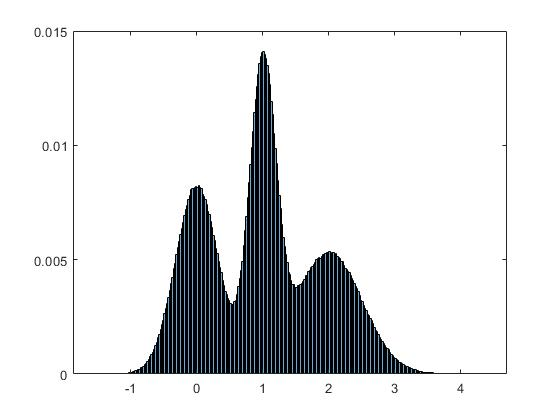
\includegraphics[width=215pt]{histGauss}
      		\caption{Normalized Histogram of 1D samples.}
		\label{fig:histGauss}
    	\end{subfigure}%
    	\begin{subfigure}[b]{0.5\linewidth}
      		\centering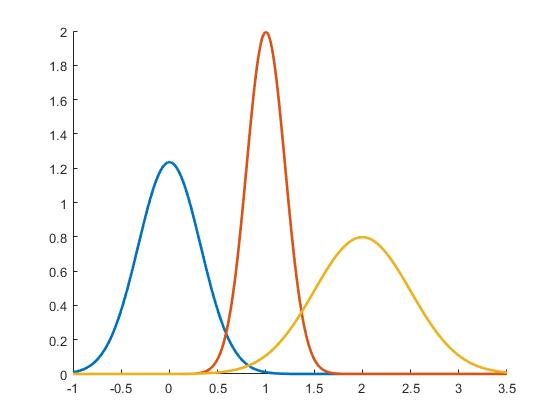
\includegraphics[width=215pt]{hist_gauss_curve}
      		\caption{Gaussians derived from 1D histogram. }
       		\label{fig:histCurve}
		\end{subfigure}
		\caption{Formulation of Mixture of Gaussians.}
    	\label{fig:mixture}
\end{figure}

With each iteration of the GMM algorithm the parameters of the model's component Gaussians are tuned according to the covariance $\ref{eq:cov}$ between samples in each cluster. 

\begin{equation}
Cov(X, Y) = \frac{\Sigma(X_i-\overline X)(Y_j-\overline Y)}{n}
\label{eq:cov}
\end{equation}

Where, $X$ and $Y$ are the variables being compared, $\overline X$ and $\overline Y$ are variable means and $n$ is the number of samples.

The algorithm seeks the highest covariance possible in each of its clusters. It is by considering the covariance of samples that the GMM is able to best classify ambiguous samples. The higher the correlation between sample dimensions the more likely it is they belong in the same cluster. This can observed in Figure \ref{fig:mogcov}, the data being clustered is the same as in Figure \ref{fig:clusters} but notice the elliptical shape of the cluster distributions as opposed to the spherical shape of K-Means clustering.

\begin{figure}[H]
	\centering
	\centering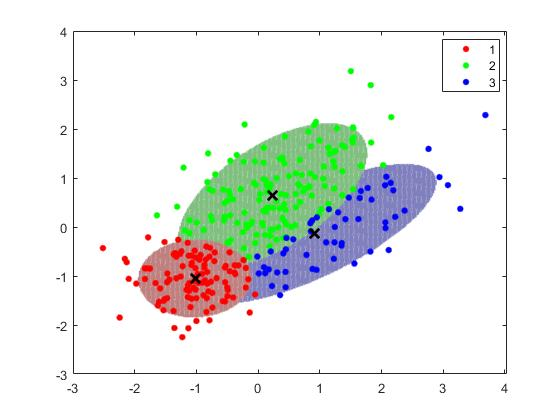
\includegraphics[width=450pt]{mog}
	\caption{Clustering using GMM.}
	\label{fig:mogcov}
\end{figure}
  
Notice the peaks in Figure \ref{fig:histScale} have been scaled such that the sum of weigthings is equal to one. This is because the probability of a sample belonging to at least one of the clusters must be equal to one. This is expressed in \ref{eq:gauss_weight1} and \ref{eq:gauss_weight2}

\begin{equation}
    0\leq \pi_k \leq 1
\label{eq:gauss_weight1}
\end{equation}
\begin{equation}
    \sum_{k=1}^{K}\pi_k = 1
\label{eq:gauss_weight2}
\end{equation}






\begin{figure}[H]
    \centering
    \centering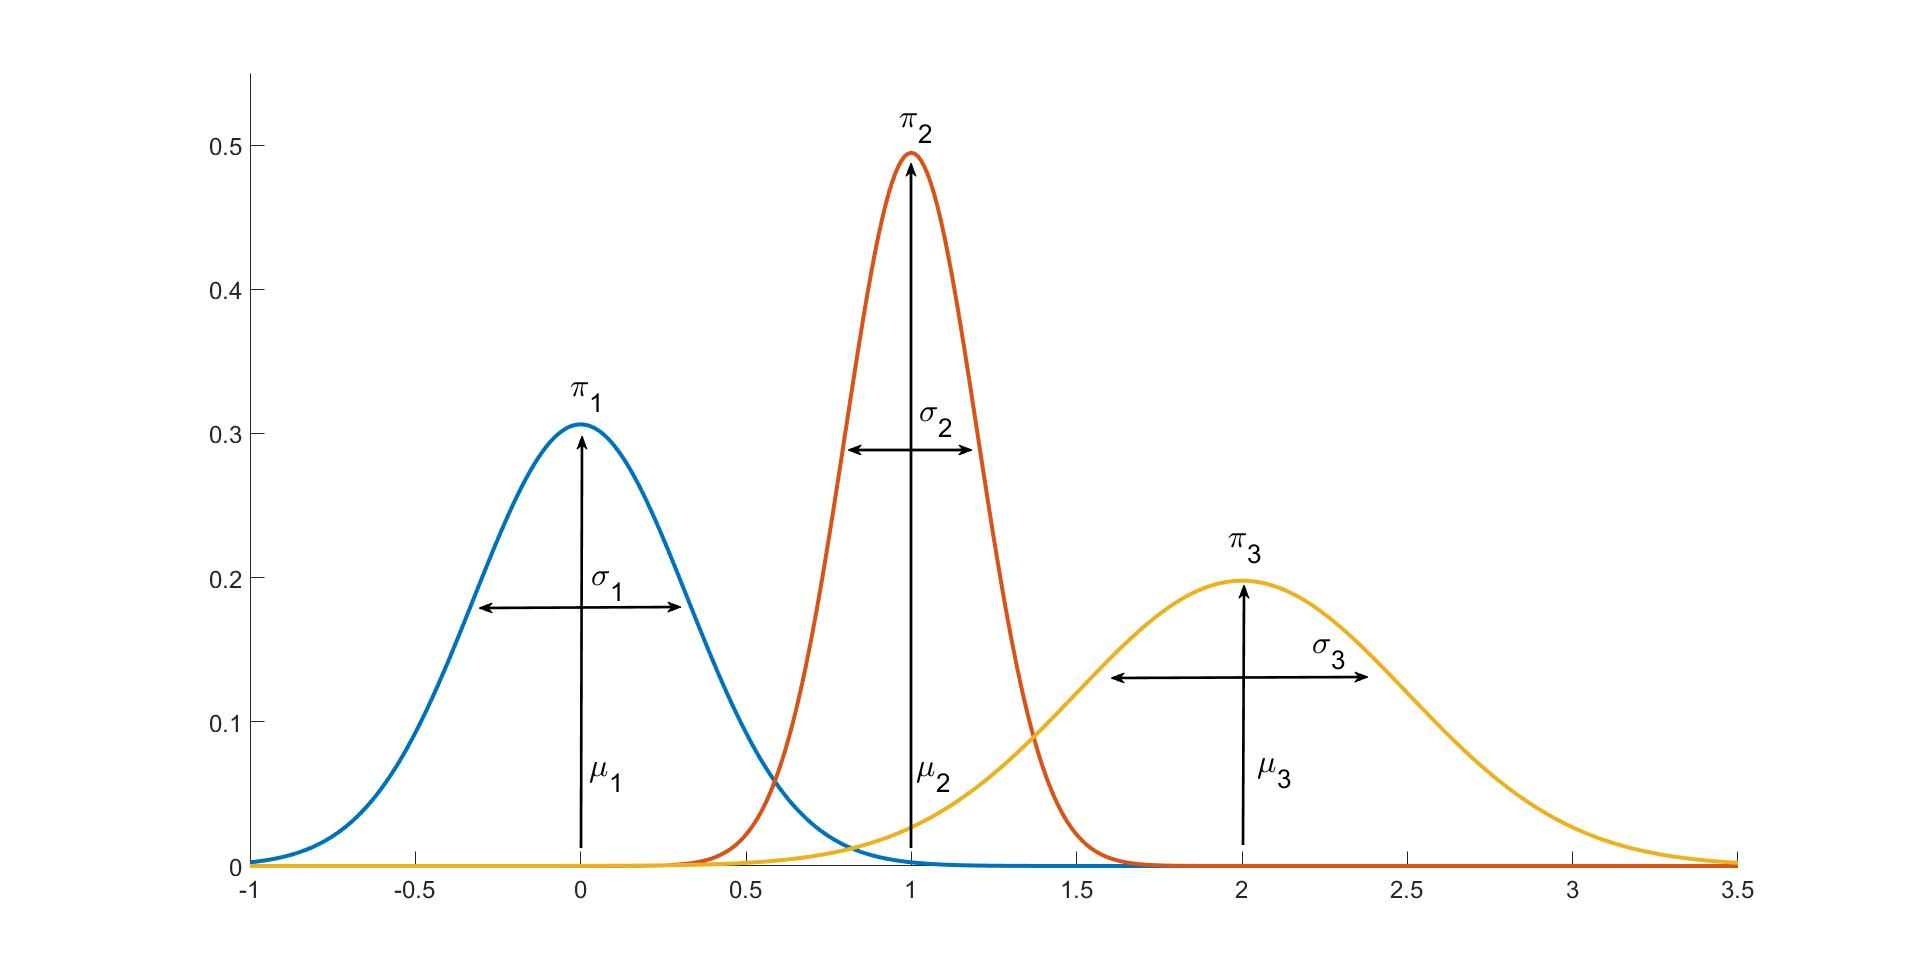
\includegraphics[width=450pt]{gauss_mix_scale}
    \caption{Individual Gaussians with scaled weightings.}
    \label{fig:histScale}
  \end{figure} 

This method is perhaps explained with an example. 




\subsubsection{Expectation Maximization}






\subsection{Background Subtraction}

This is performed by identifying a background image and then subtracting this image from subsequent frames of video to determine what has changed and hence what is a foreground image.

\subsection{Expectation Maximization}

This is an optimization scheme used to fit a Gaussian Mixture Model. It is an iterative method that faurantees convergence to a local maximum in a search space.